\section{Agentic 3D, CAD, and World Generation}
\label{sec:3d-cad-world}

Three-dimensional creation makes state more explicit but also makes visual plausibility an insufficient success criterion. Geometry, topology, dimensions, joints, scene graphs, operation histories, collisions, and simulator outcomes can all be inspected, so agents can act on executable structure rather than pixels alone. This section separates appearance-oriented world construction from editable CAD and from verification-driven refinement.

\begin{figure}[!htbp]
  \centering
  
\definecolor{avgmapblue}{HTML}{22558A}
\definecolor{avgmapgreen}{HTML}{23845D}
\ifdefined\avgmapfont\else\newcommand{\avgmapfont}{\rmfamily}\fi
\makebox[\linewidth][c]{%
\resizebox{0.98\linewidth}{!}{%
\begin{tikzpicture}[
  avg branch/.style={draw=avgmapblue!58, fill=avgmapblue!9, text=black!88, rounded corners=2.5pt, line width=0.48pt, text width=42mm, minimum height=10.5mm, align=center, inner xsep=2.2mm, inner ysep=0.9mm, outer sep=0pt, execute at begin node={\hyphenpenalty=10000\exhyphenpenalty=10000\relax}, font=\avgmapfont\fontsize{7.35}{8.35}\selectfont\bfseries},
  avg papers/.style={draw=avgmapblue!25, fill=avgmapblue!2, text=black!88, rounded corners=2.5pt, line width=0.38pt, text width=115mm, minimum height=10.5mm, align=left, inner xsep=3mm, inner ysep=0.9mm, outer sep=0pt, execute at begin node={\hyphenpenalty=10000\exhyphenpenalty=10000\relax}, font=\avgmapfont\fontsize{7.15}{8.25}\selectfont\bfseries},
  avg benchmark branch/.style={avg branch, draw=avgmapgreen!78, fill=avgmapgreen!15, text=avgmapgreen!45!black},
  avg benchmark papers/.style={avg papers, draw=avgmapgreen!72, fill=avgmapgreen!7, text=black!88},
  avg root/.style={draw=avgmapblue, fill=avgmapblue!94!black, text=white, rounded corners=2.5pt, line width=0.55pt, minimum width=9mm, minimum height=36mm, inner sep=0pt, outer sep=0pt},
  avg line/.style={draw=black!28, line width=0.45pt, line cap=round},
  avg benchmark line/.style={draw=avgmapgreen!78, line width=0.55pt, line cap=round}
]
\matrix (avgmap) [matrix of nodes, row sep=1.35mm, column sep=3mm, ampersand replacement=\&, nodes={anchor=center}] {
  \node[avg branch] (c6b1) {Scene Graphs and Worlds}; \& \node[avg papers] (c6p1) {ShapeCraft~\cite{avg251017603}, Idea23D~\cite{avg240404363}, WorldCraft~\cite{avg250215601}, WorldAgents~\cite{avg260319708}, SimWorlds~\cite{avg260701766}.}; \\
  \node[avg branch] (c6b2) {Executable CAD}; \& \node[avg papers] (c6p2) {From Idea to CAD~\cite{ocker2025ideatocad}, ArtiCAD~\cite{avg260410992}, CAD-Assistant~\cite{mallis2024cadassistant}, CADReasoner~\cite{kabisov2026cadreasoner}, IterCAD~\cite{hu2026itercad}.}; \\
  \node[avg branch] (c6b3) {Geometry-Aware Verification}; \& \node[avg papers] (c6p3) {CAD-Judge~\cite{zhou2025cadjudge}, Physics-in-the-Loop~\cite{avg260519717}, TOOLCAD~\cite{gong2026toolcad}, CADSmith~\cite{barkley2026cadsmith}, CLARE~\cite{avg260716352}.}; \\
  \node[avg benchmark branch] (c6b4) {Benchmarks}; \& \node[avg benchmark papers] (c6p4) {PhysCodeBench~\cite{xie2026physcodebench}, 3DCodeBench~\cite{avg260601057}.}; \\
};
\coordinate (c6trunktop) at ($(c6b1.west)+(-4.6mm,0)$);
\coordinate (c6trunkbottom) at ($(c6b4.west)+(-4.6mm,0)$);
\coordinate (c6rootnw) at ($(c6b1.north west)+(-15.5mm,0)$);
\coordinate (c6rootse) at ($(c6b4.south west)+(-7.6mm,0)$);
\node[avg root, fit=(c6rootnw)(c6rootse)] (c6root) {};
\node[rotate=90, align=center, text=white, font=\avgmapfont\fontsize{7.05}{8.15}\selectfont] at (c6root.center) {{\bfseries CHAPTER 6}\\[0.55mm]{\fontsize{6.2}{7.15}\selectfont 3D, CAD, and worlds}};
\draw[avg line] (c6trunktop) -- (c6trunkbottom);
\coordinate (c6trunkmid) at ($(c6trunktop)!0.5!(c6trunkbottom)$);
\draw[avg line] (c6root.east) -- (c6trunkmid);
\draw[avg line] (c6trunktop |- c6b1.west) -- (c6b1.west);
\draw[avg line] (c6b1.east) -- (c6p1.west);
\draw[avg line] (c6trunktop |- c6b2.west) -- (c6b2.west);
\draw[avg line] (c6b2.east) -- (c6p2.west);
\draw[avg line] (c6trunktop |- c6b3.west) -- (c6b3.west);
\draw[avg line] (c6b3.east) -- (c6p3.west);
\draw[avg benchmark line] (c6trunktop |- c6b4.west) -- (c6b4.west);
\draw[avg benchmark line] (c6b4.east) -- (c6p4.west);
\end{tikzpicture}%
}%
}

  \caption{Representative systems and benchmarks for agentic 3D, CAD, and world generation, organized according to the chapter taxonomy.}
  \label{fig:ch6-representative-systems}
\end{figure}

\subsection{Scene graphs, assets, layouts, and interactive worlds.}
World construction combines asset selection, spatial arrangement, scene-graph state, and sometimes simulation. The key distinction is whether an agent merely writes a scene description or can observe and revise the instantiated world.

\paragraph{Multi-agent Evolutionary Systems for the Generation of Complex Virtual Worlds}
This early study combines an Interactive Genetic Algorithm with a learning agent for procedural city generation: a human selects preferred cityscapes while a J48 decision-tree agent observes those choices and incrementally learns to select candidates on the user's behalf, gradually shifting control to mitigate fatigue~\cite{avg160405792}. Across 36 runs, the agent-assisted method used more total generations but roughly half the human evaluations compared to the IGA. 


\paragraph{Genie} trains an 11B-parameter foundation world model on 30,000 hours of unlabeled Internet gameplay videos: a spatiotemporal video tokenizer, a MaskGIT dynamics model, and a fully unsupervised latent action model together turn a single text, image, or sketch prompt into an action-controllable environment that is stepped through frame by frame~\cite{avg240215391}. The learned latent action space further lets agents imitate behaviors from action-free videos, though the in-loop decisions remain with the human or downstream agent rather than the model itself.

\paragraph{GameNGen} replaces the hand-written game loop with a neural engine: an RL agent first plays DOOM to record training sessions, then an augmented Stable Diffusion v1.4 learns next-frame prediction conditioned on past frames and actions, with noise augmentation stabilizing long autoregressive rollouts~\cite{valevski2024gamengen}. The engine simulates playable DOOM at 20 FPS on a single TPU and persists game state---health, ammo, doors---over multi-minute trajectories, but the action stream still comes from the player, so the system supplies an interactive world rather than agentic decisions.

\paragraph{Genie 2} scales the generative-interactive-environment paradigm to rich 3D worlds: an autoregressive latent diffusion model with a causal-masked transformer dynamics model turns a single prompt image into a playable environment that responds to keyboard and mouse actions frame by frame, sustaining consistent worlds for up to a minute with emergent physics, object affordances, NPC behavior, and long-horizon memory of off-screen regions~\cite{parkerholder2024genie2}. A SIMA agent can be placed inside the generated world to follow natural-language instructions, so the model supplies the interactive environment while task-level decisions remain with the embedded agent or human player.

\paragraph{ShareVerse} targets multi-agent shared world modeling in video generation: four-view videos of independent agents are spatially concatenated to cover a broader environment with internal multi-view geometric consistency, while cross-agent attention blocks injected into a pretrained video model transmit spatiotemporal information across agents so that overlapping regions stay consistent and non-overlapping regions remain plausible~\cite{avg260302697}. A CARLA-built dataset of diverse scenes, weather conditions, and paired multi-view trajectories supports 49-frame generation that tracks dynamic agents across views.

\paragraph{MultiWorld} scales action-conditioned video world models to multi-agent, multi-view settings: a Multi-Agent Condition Module gives precise per-agent control, a Global State Encoder keeps observations coherent across views, and all views are synthesized in parallel so that agent and view counts scale flexibly~\cite{avg260418564}. On multi-player game environments and multi-robot manipulation tasks, it improves video fidelity, action-following, and multi-view consistency over baselines.

\paragraph{MetaWorld} scales multi-agent world modeling from single-view videos alone: Monocular World-State Unrolling decomposes monocular footage into camera ego-motion and subject trajectories, extracting synchronized multi-agent motion in a shared 3D space without multi-camera recordings; a Subject-Aware World Generator conditions simulation on per-agent identity images; and World-State Alignment---per-frame inter-branch cross-attention at every DiT layer---synchronizes denoising so that both egocentric views stay grounded in the same physical reality~\cite{avg260602753}.

\paragraph{Prisma-World} formulates multi-agent world generation as a joint geometry-aware denoising process: all agent videos are processed within one full-attention sequence, a multi-agent RoPE distinguishes agent identities under synchronized temporal coordinates, and relative camera geometry injected into attention biases overlapping viewpoints toward shared scene evidence~\cite{avg260609507}. An overlap-decaying curriculum and minimap-conditioned structural guidance further strengthen cross-view consistency, supported by PrismaDataset, a large-scale UE5 dataset with composable multi-agent view groups and precise camera/action annotations.

\paragraph{OmniDrive} recasts controllable multi-view driving video generation as LLM-choreographed latent choreography: three Qwen2.5-VL agents---a Director parsing user intent into a structured WorldScript, a Cartographer grounding it into spatially anchored layout tokens, and an Auditor feeding cross-view critiques back as auxiliary supervision---jointly author a single position-aware token sequence that is co-compressed with multi-view video through a view-time permutation inside a 3D VAE~\cite{avg260617536}. On nuScenes it reports state-of-the-art multi-view consistency and BEV mAP, and a detector trained purely on its synthetic data gains +2.4 NDS on the real validation split.

\paragraph{WorldWeaver} augments streaming multi-agent autoregressive video diffusion with world state registers: learnable tokens that store shared world information, track individual agent status, and are dynamically updated after each generated chunk, supervised by signals spanning agent status, bird's-eye views, and scene text, while a Mixture-of-Transformers separates world-state modeling from visual frame modeling~\cite{avg260721594}. On two-agent Minecraft generation, explicit world-state modeling improves logical consistency and generation quality, giving the world model a persistent state that carries across agents and views.

\paragraph{ShapeCraft}
 uses a multi-agent system with a Graph-based Procedural Shape representation to generate structured, editable 3D assets: Parser, Coder, and Evaluator agents decompose text into semantic components, iteratively render, score, and refine candidate geometries, with component-aware texture applied post-construction~\cite{avg251017603}. Figure~\ref{fig:ch6-structured-assets} illustrates this component-level construction process.

\begin{figure}[!htbp]
  \centering
  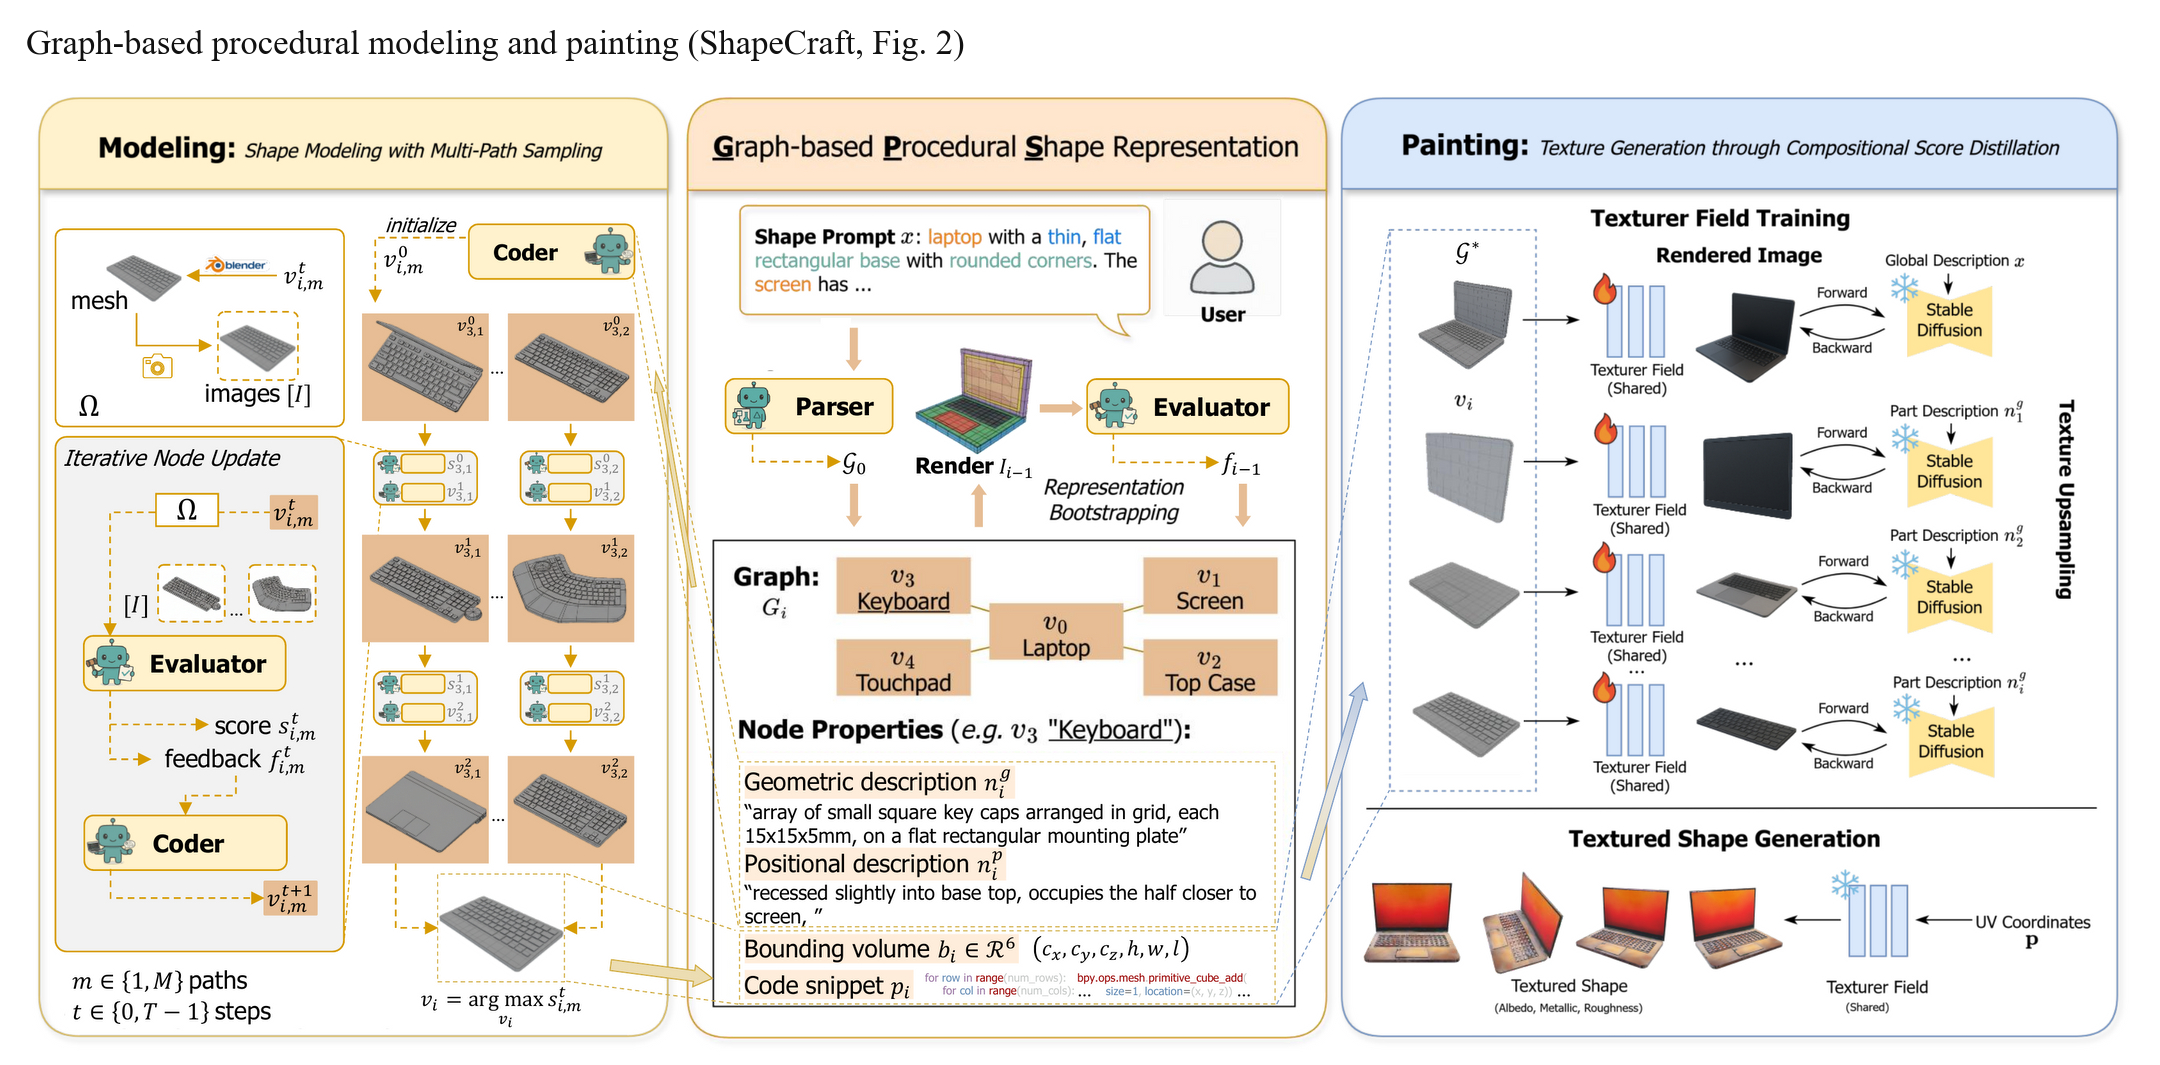
\includegraphics[width=\textwidth]{figures/ch6_structured_editable_3d_assets.jpg}
  \caption{Structured 3D asset generation. ShapeCraft decomposes a requested object into a graph of semantic components whose bounding volumes, executable code, rendered geometry, and textures are iteratively constructed and refined~\cite{avg251017603}.}
  \label{fig:ch6-structured-assets}
\end{figure}

\paragraph{Agentic Designer} progressively decomposes an interior layout among agents and applies structure-aware checks after each stage, so invalid spatial arrangements are corrected before detailed rendering~\cite{avg260720866}.

\paragraph{Authoring for Living Worlds}
Tool-constrained LLM agents author executable multi-actor event graphs for a 3D world: a Director explores a capability registry and delegates scenes to a Scene Builder that constructs per-actor chains through validated tools against a transactional state backend, emitting only valid specifications by construction~\cite{avg260410383}. A six-stage GPT-5 pipeline produced zero executables in 50 attempts. The system's visual output is bounded by the engine's fixed cameras.

\paragraph{CoGen3D} keeps user intent, design memory, and iterative choices in a human--AI co-design loop for virtual-reality assets rather than automating away creative authority~\cite{avg260703731}.

\paragraph{MA3DSG} addresses the scalability challenge in 3D scene graph generation by distributing object, relation, and scene-graph construction across multiple agents, targeting large indoor environments that exceed the capacity of conventional single-agent systems~\cite{avg260204152}.

\paragraph{One Sentence, One Drama} maintains character, set, and event state while agents plan and critique a personalized short drama, using 3D-grounded first-frame generation to enforce cross-clip spatial consistency~\cite{avg260522144}.

\paragraph{OrchestrXR}
 uses three specialized agents to progressively transform XR research ideas into structured study, scene, and interaction specifications, with live Unity streaming for grounded user feedback and revision~\cite{avg260701588}. A user study with 12 researchers shows strong intent preservation (SPS=0.86) and positive usability (SUS=79.17), though design-to-scene grounding remains the main bottleneck. 

\paragraph{WorldAgents}
 uses a multi-agent framework—Director, Generator, and two-stage Verifier—to extract navigable 3D worlds from 2D image foundation models via iterative inpainting and 3D-consistent verification~\cite{avg260319708}. The system relies on VLM judgments, inherits geometric drift, and follows a fixed left/right exploration policy.

\paragraph{Idea23D} generates 3D models from interleaved multimodal inputs (text, images, and 3D models) through three LMM-based agents for prompt generation, model selection, and feedback refinement. The Prompt Generator converts multimodal IDEAs into text prompts; the Model Selector picks the best 3D candidate via multiview rendering; the Feedback Refiner analyzes gaps and suggests improvements. A memory module stores history to guide iterations. ~\cite{avg240404363}.

\paragraph{MuMA} decouples PBR texturing into multi-view shaded and albedo generation, then leverages an intrinsic decomposition model to recover metallic and roughness, with a VLM agent scoring and selecting between generated and decomposed albedo candidates~\cite{avg250318461}.

\paragraph{RAISECity} retrieves real-world geographic and visual evidence, uses multimodal agents to imagine complete building appearances from incomplete observations, generates city-scale 3D content aligned to OSM layouts, and applies iterative VLM-based reflection and refinement to correct geometric and semantic deviations between generated worlds and their real references~\cite{avg251118005}.

\paragraph{WorldCraft} uses LLM agents to plan assets via a self-growing manual that masters procedural generators, and to arrange layouts via hierarchical numerical optimization with ergonomic and aesthetic constraints~\cite{avg250215601}.

\paragraph{A Multi-Agent Framework for Democratizing XR Content Creation in K--12 Classrooms} assigns ideation and content-construction roles to agents while keeping teachers and students in control, lowering the tooling barrier to executable classroom experiences~\cite{avg260404728}.

\paragraph{Articraft} generates articulated assets through executable code and stores generation traces for future fine-tuning, providing a scalable path from static 3D shapes to movable structures~\cite{avg260515187}.

\paragraph{Metric-Guided Synthetic Rendering} generates synthetic image data via procedural rendering and modulates scene parameters under task metrics, making downstream learning utility part of the objective~\cite{avg260712874}.

\paragraph{NaLA} is a 3D-native layout agent that takes point-cloud geometry as input and predicts poses directly, avoiding the loss introduced when spatial decisions are mediated through 2D renderings or text~\cite{avg260629395}.

\paragraph{PhysCodeBench} provides a benchmark for physics-aware symbolic simulation, while SMRF uses self-corrective multi-agent refinement to repair violated physical constraints~\cite{xie2026physcodebench}.

\paragraph{SceneConductor} constructs 3D scenes from a single image via geometry-aware layout prediction and environmental scaffolding, then refines the scene through planner-directed simple fixes and specialist-isolated complex corrections~\cite{avg260608402}.

\paragraph{SimWorlds} plans assets and dynamics through a staged construction pipeline, then verifies each stage against Blender engine state—modifier stacks, physics caches, and collision relations—rather than rendered images alone, enabling mechanism-correct 4D scene generation that visual-only critics cannot ensure~\cite{avg260701766}.

\paragraph{Vinedresser3D} decomposes text-guided 3D edits into localized asset operations, supporting precise modification of existing scenes rather than full regeneration~\cite{avg260219542}.

\paragraph{AGILE: Hand--Object Interaction Reconstruction from Video via Agentic Generation} reconstructs simulation-ready hand-object interaction assets from monocular video via VLM-guided generation and contact-aware optimization, producing watertight meshes and 6D pose trajectories rather than visually plausible renderings~\cite{avg260204672}.

\subsection{Executable CAD programs and editable solids.}
CAD makes action history and constraints first-class. Code, sketches, feature operations, and parametric edits provide precise interventions, while rendered views offer complementary visual evidence that the underlying solid remains meaningful.

\paragraph{CrossMatAgent} automates metamaterial design via a four-agent team (Describer, Architect, Builder, Supervisor) that analyzes input patterns and iteratively refines DALL-E 3 prompts through supervisor-guided reflection. The resulting 700 image-text pairs fine-tune SDXL with CLIP alignment, generating 2D patterns that are binarized and path-connected by design—not post-hoc—enabling direct use in simulation meshing and 3D printing slicers without heuristic repair, though outputs remain raster patterns rather than parametric CAD or editable solids~\cite{avg250319889}.

\paragraph{From Idea to CAD}
converts sketches, photos, and text into parameterized CadQuery models via a three-agent team—Requirements Engineer, CAD Engineer, and Quality Assurance Engineer—that iteratively clarifies specifications, generates and repairs code with compiler feedback, and verifies outputs against multi-view renderings, with user confirmation as an outer validation loop~\cite{ocker2025ideatocad}.

\paragraph{Agent-Aided Design for Dynamic CAD Models} targets the "scissors test"—generating 3D assemblies with moving parts and revolute joints—by having an agent write JSON definitions for parts, links, and degrees-of-freedom, compiled through a modified multibody constraint solver with quaternion-based orientation and FreeCAD rendering. Unlike prior static CAD generation, the agent iteratively repairs joint definitions using solver errors and uniquely colored per-instance renderings that disambiguate identical components.~\cite{avg260415184}.

\paragraph{ArtiCAD}
 generates editable, articulated CAD assemblies from text or images via a four-agent system that introduces Connectors—explicit attachment points with joint types and local frames—specified at design time rather than inferred during assembly, reducing connection matching to deterministic alignment. Per-part scripts are generated with local validation; assembly occurs without LLM calls; cross-stage rollback isolates design versus code errors.~\cite{avg260410992}

\paragraph{Clarify Before You Draw}
ProCAD decomposes text-to-CAD into proactive clarification followed by code synthesis, addressing prompts with missing or conflicting dimensions via a clarification agent that asks targeted questions in a single turn before passing a standardized specification to a fine-tuned CadQuery coder~\cite{avg260203045}. On ambiguous prompts, ProCAD substantially outperforms direct Claude Sonnet 4.5 in Chamfer distance and invalidity; human evaluation on 100 examples confirms the trend. 

\paragraph{Zero-to-CAD}
 synthesizes executable, editable CAD construction sequences at scale without real design histories, using an LLM with tool access that iteratively generates code, validates geometry, and consults documentation to repair errors~\cite{avg260424479}. The pipeline produces nearly one million sequences covering Booleans, fillets, chamfers, shells, and sweeps, with fine-tuned models demonstrating strong generalization to human-designed CAD and outperforming frontier VLMs on reconstruction tasks.

\paragraph{CAD-Assistant} is a training-free, general-purpose CAD agent that augments a VLLM with FreeCAD tools—execution, rendering, constraint checking, and cross-section extraction—to iteratively plan and revise open-ended design tasks from sketches, scans, or text, moving beyond dataset-bound or task-specific generation~\cite{mallis2024cadassistant}. Figure~\ref{fig:ch6-cad-feedback} summarizes the task coverage supported through this executable interface.

\begin{figure}[!htbp]
  \centering
  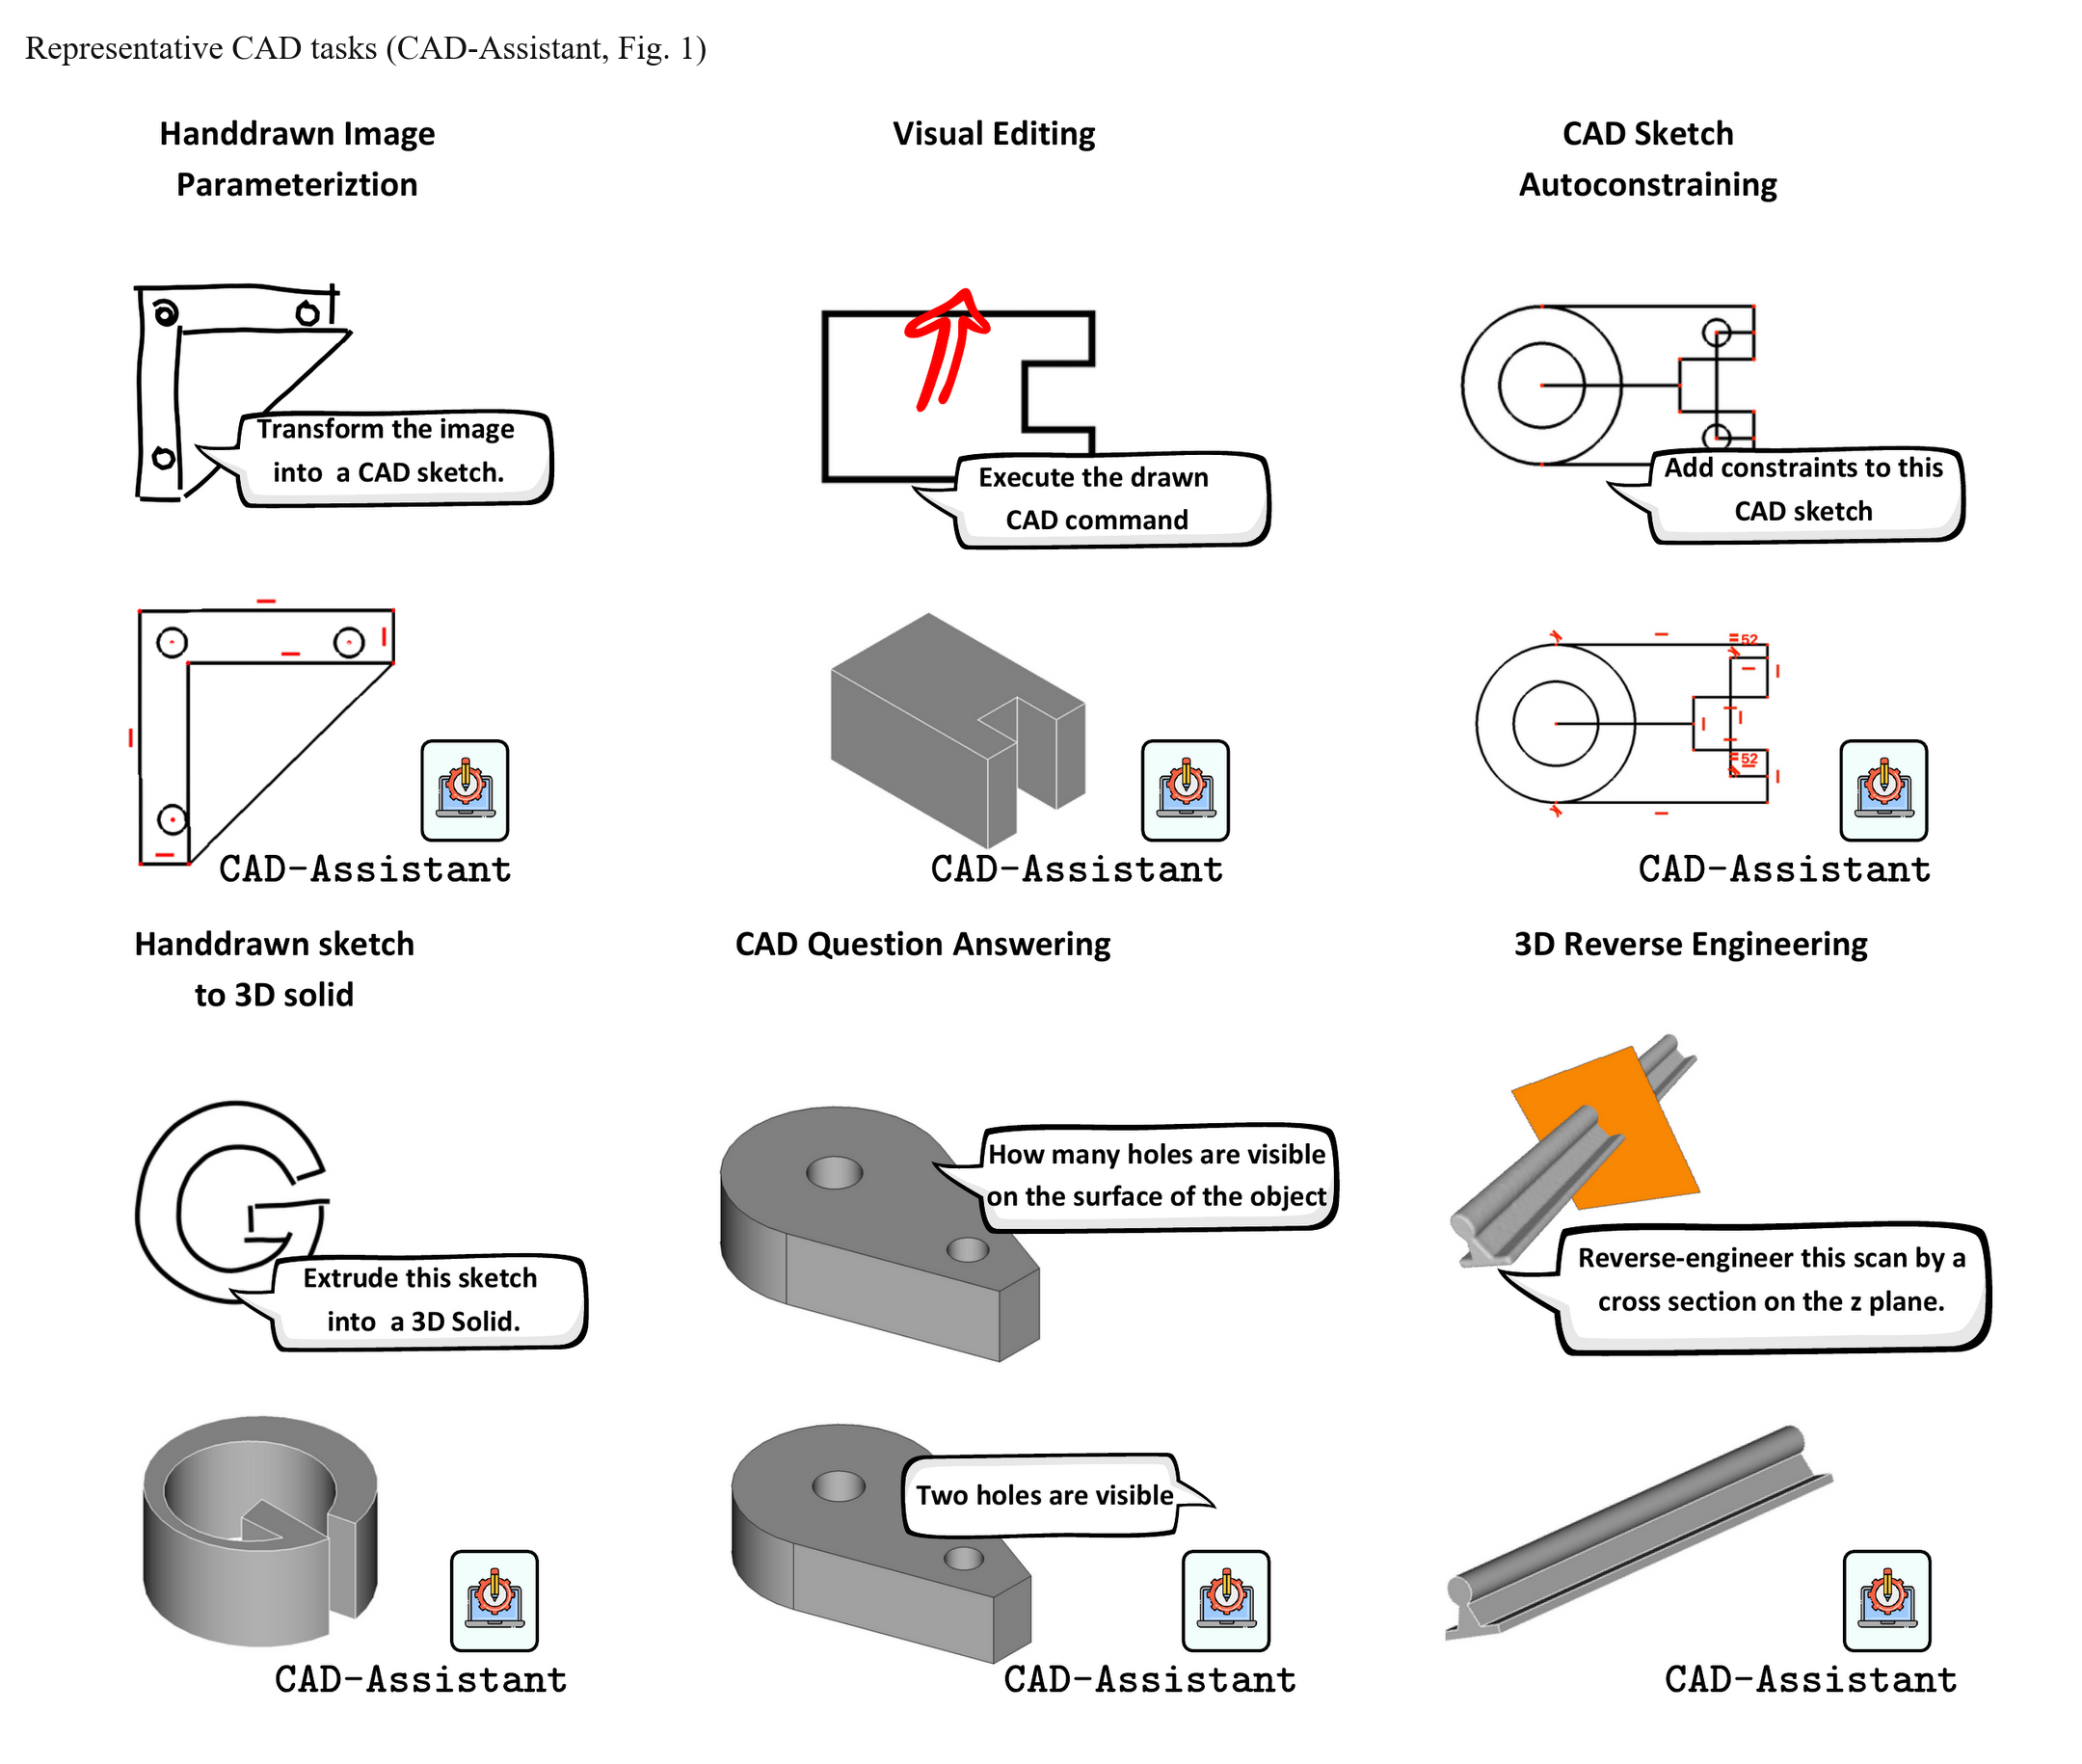
\includegraphics[width=\textwidth]{figures/ch6_executable_cad_feedback.jpg}
  \caption{Representative task coverage of CAD-Assistant across sketch parameterization, visual editing, constraint construction, solid generation, question answering, and reverse engineering~\cite{mallis2024cadassistant}.}
  \label{fig:ch6-cad-feedback}
\end{figure}

\paragraph{CADReasoner} frames scan-to-CAD as iterative self-editing: a single model compares rendered geometry with the target via multi-view overlays and point-cloud offsets, then rewrites its own CadQuery program to close the gap, learning to correct from its own prediction errors without RL or frozen VLMs~\cite{kabisov2026cadreasoner}.

\paragraph{IterCAD} unifies generation and editing as a closed-loop agent that parses dimensioned engineering drawings and refines CadQuery code using sandbox feedback—compiler logs and OCCT-projected views with explicit dimensions—to localize errors to specific sketch entities rather than global shape discrepancies. Progressive SFT and GSPO with Geometry-Viable Prefix Masking instill self-correction without penalizing early correct turns for downstream failures~\cite{hu2026itercad}.

\subsection{Geometry-aware verification, simulation, and learning.}
Verification can inspect geometry, physics, compilation, and task function independently of appearance. These signals also make 3D a useful setting for reinforcement learning and self-corrective search.

\paragraph{CAD-Judge}
replaces VLM-based rendering and ranking with a local CAD compiler that reconstructs B-reps or meshes and supplies Chamfer-distance and compilation signals as fast, rule-based rewards during preference alignment, while a Compiler-as-a-Review module appends syntax, closure, extrusion, or Boolean errors to the prompt for iterative regeneration at inference~\cite{zhou2025cadjudge}.  

\paragraph{Physics-in-the-Loop}
 embeds FEA as a deterministic verification signal into an agentic CAD loop, where a multi-agent system iteratively generates and refines designs until they pass geometry and physics checks for load-bearing validity, rather than optimizing geometric similarity alone~\cite{avg260519717}. Figure~\ref{fig:ch6-physics-verification} shows how geometric and finite-element evidence returns to planning and code generation.

\begin{figure}[!htbp]
  \centering
  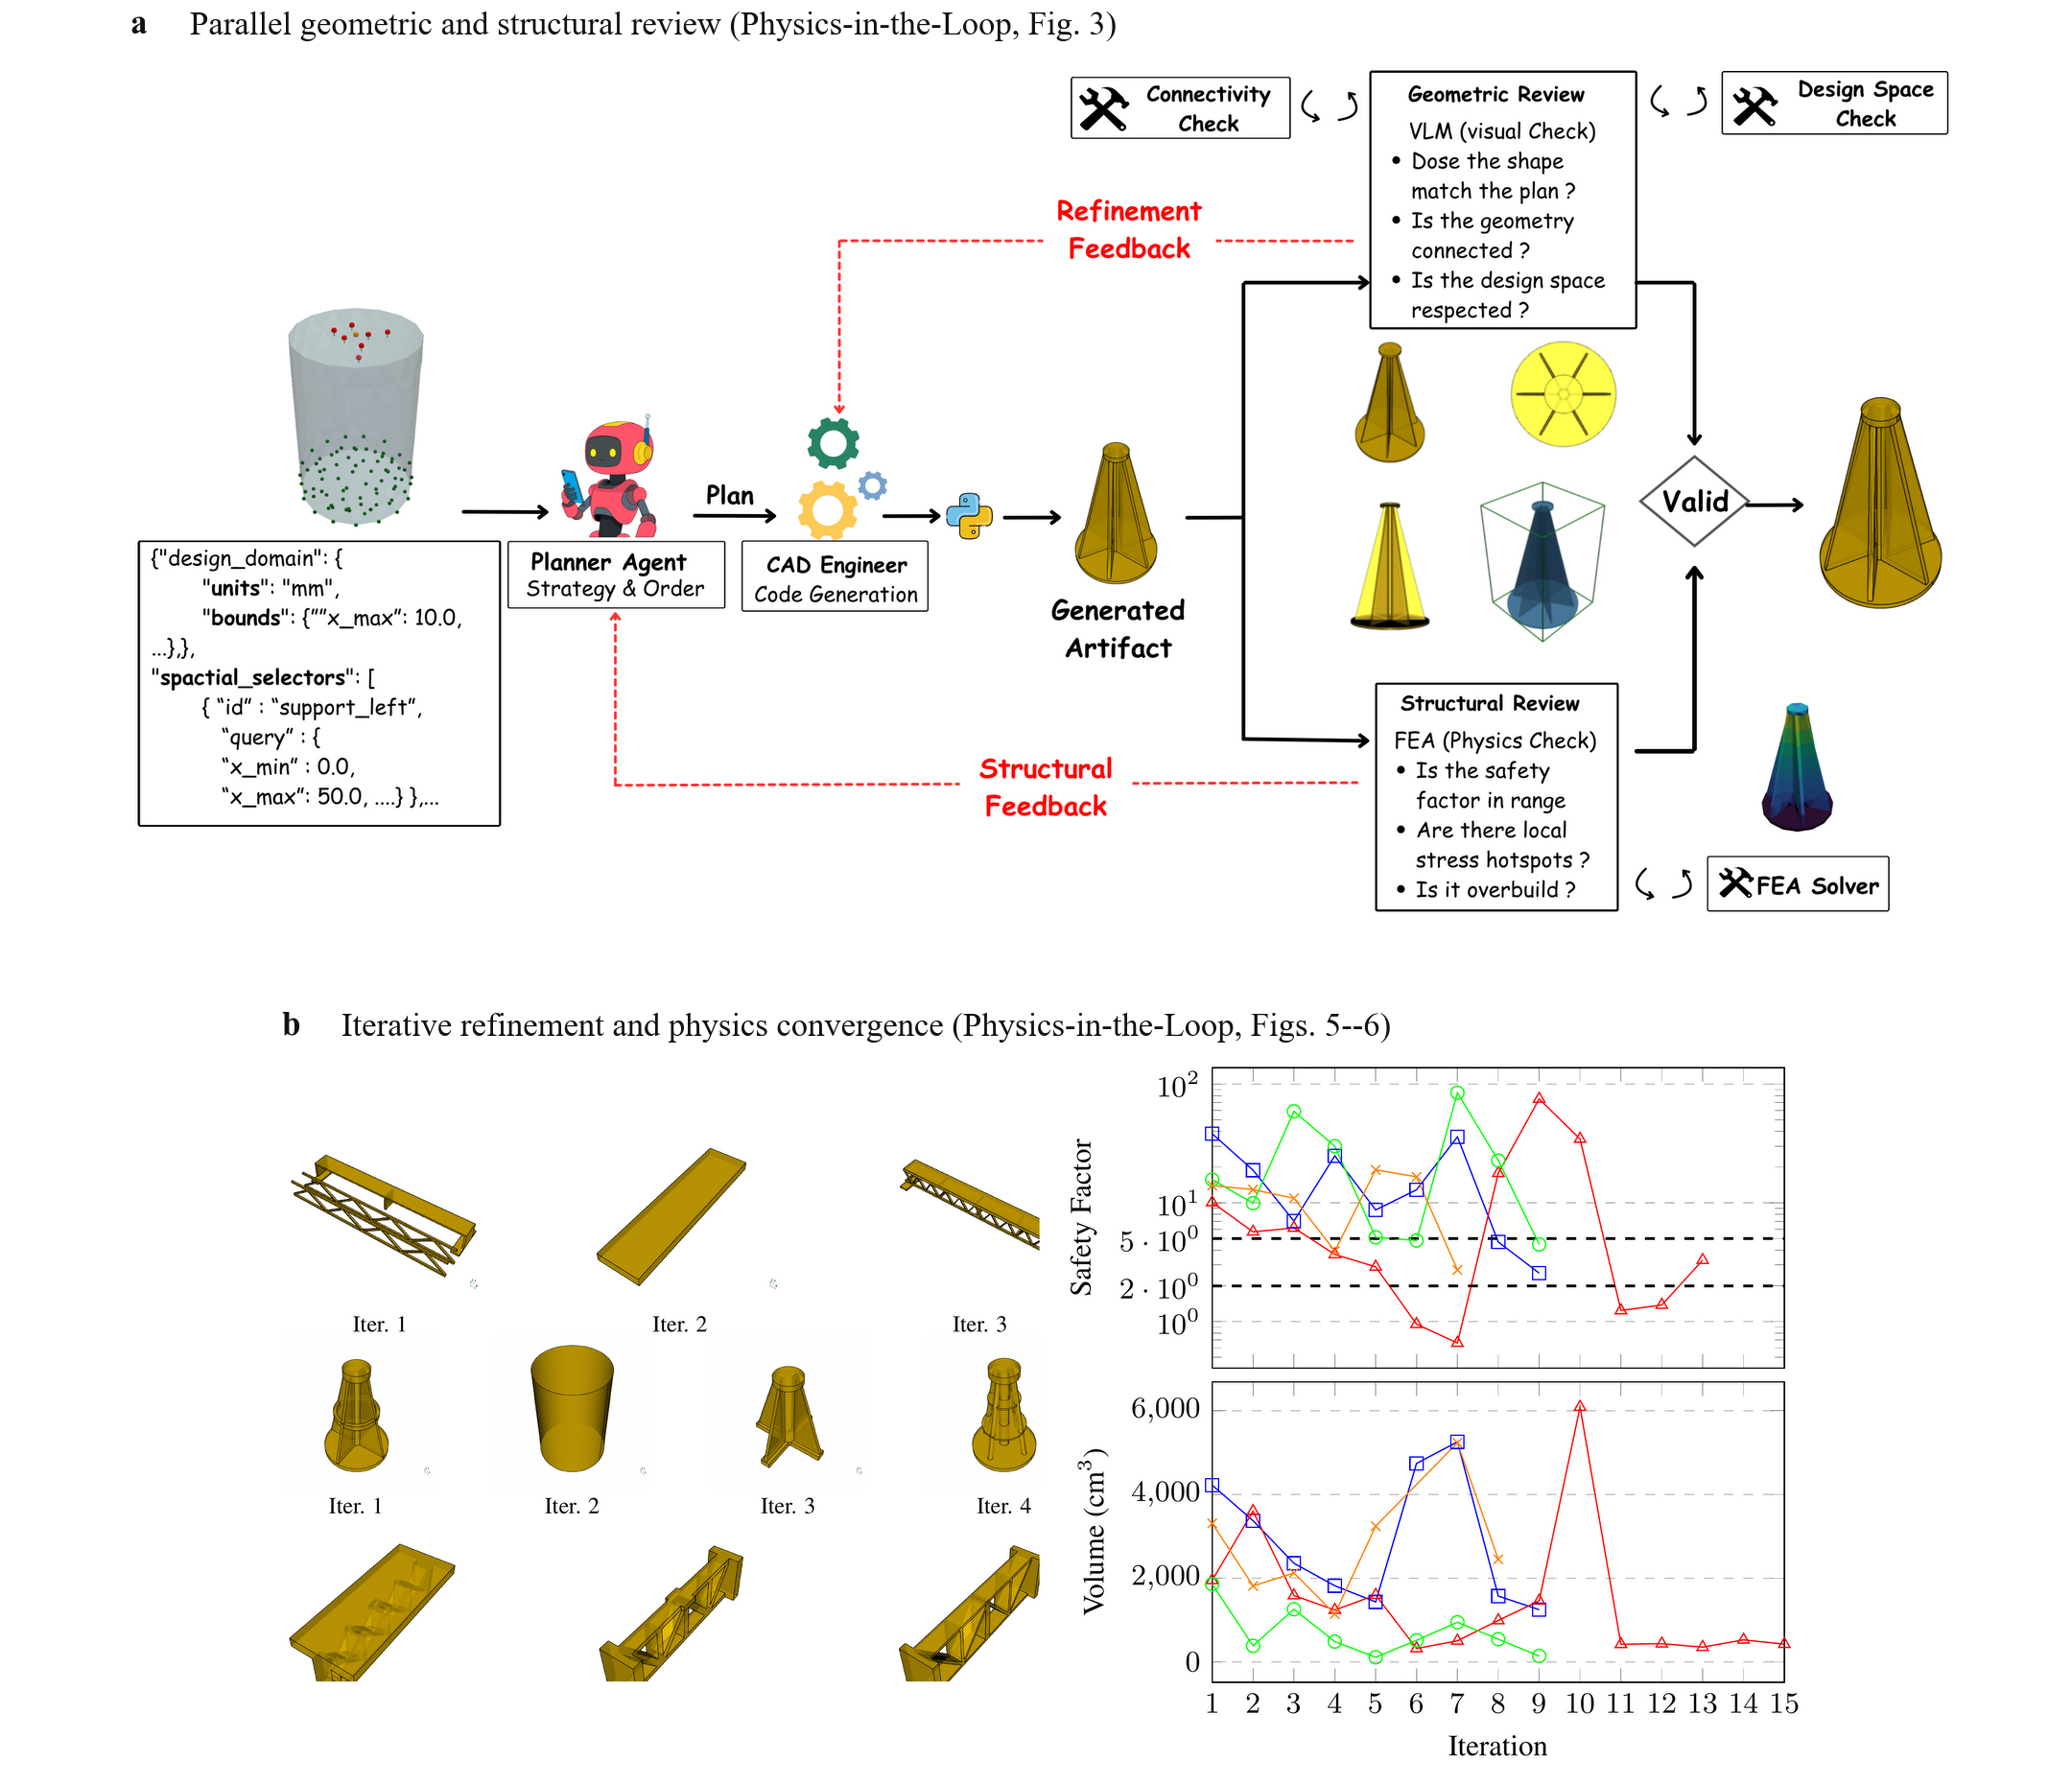
\includegraphics[width=\textwidth]{figures/ch6_physics_grounded_verification.jpg}
  \caption{Geometry- and physics-grounded verification. Physics-in-the-Loop sends each generated CAD artifact to parallel geometric and finite-element reviewers, routes their feedback back to planning and code generation, and iteratively moves candidate designs toward valid geometry and target structural behavior~\cite{avg260519717}.}
  \label{fig:ch6-physics-verification}
\end{figure}



\paragraph{TOOLCAD}
 trains open-source LLMs as tool-using CAD agents via online reinforcement learning, where a ReAct-style policy interacts with FreeCAD through MCP-based primitives and receives step-level engine feedback (exceptions, constraint warnings, success/failure) plus trajectory-level outcome rewards from a trained ORM, updated with GRPO across a part-wise curriculum~\cite{gong2026toolcad}. 


\paragraph{3D Furniture Layout RL}
decompose 3D furniture layout into two coupled 2D control problems (x-y and y-z planes) and train cooperative DQN agents to move furniture under IoU-based geometric rewards, producing 3D layouts that outperform prior 2D-only methods on indoor scene benchmarks~\cite{avg210209137}.

\paragraph{CADSmith} combines RAG-augmented code generation with programmatic geometric validation via OpenCASCADE kernel metrics (volume, bounding box dimensions, face counts, solid validity) and an independent VLM Judge with three-view renders, triggering iterative refinement through nested execution and geometry correction loops~\cite{barkley2026cadsmith}.

\paragraph{CLARE} proactively gates 3D tool execution by detecting ambiguity, missing information, and mistaken details, then learns clarification policies through simulated user interactions and Multi-turn Reward optimization to balance task success against interaction~\cite{avg260716352}.


\paragraph{3DCodeBench} provides a benchmark and human-preference arena for evaluating VLM agents on procedural 3D modeling via Blender Python code, measuring executability, multi-view perceptual similarity, and 3D geometric alignment across 212 categories, while multi-turn error feedback reveals that API fixes lift executability but do not improve shape fidelity~\cite{avg260601057}.


Three-dimensional domains offer unusually strong heterogeneous evidence, yet the evidence is split across rendered appearance, geometric validity, editability, and physical function. A convincing agent must preserve all four views of state and repair the underlying representation rather than optimizing only a camera projection.

\FloatBarrier
